\documentclass{beamer}
\usetheme{Madrid} % My favorite!
\setbeamercovered{invisible}
% To remove the navigation symbols from 
% the bottom of slides%
\setbeamertemplate{navigation symbols}{} 
%
\usepackage{graphicx}
\usepackage{subfig}
\graphicspath{{figures/}}

%\usepackage{bm} % For typesetting bold math (not \mathbold)
%\logo{\includegraphics[height=0.6cm]{yourlogo.eps}}
%
\title[Anchor Placement]{Anchor Node Placement for Localization in Wireless Sensor Networks}
\author{Ben Tatham}
\institute[Carleton University]
{
Carleton University \\
Ottawa-Carleton Institute for
Electrical and Computer Engineering \\
\emph{tatham@ieee.org}
}
\date{January 19, 2011}
% \today will show current date. 
% Alternatively, you can specify a date.
%
\begin{document}
%
\begin{frame}
\titlepage
\end{frame}
%
\begin{frame}{Motivation}
\begin{block}
{Why Wireless Sensor Networks?}
\begin{figure}
  \centering
	\subfloat[Great Duck Island]{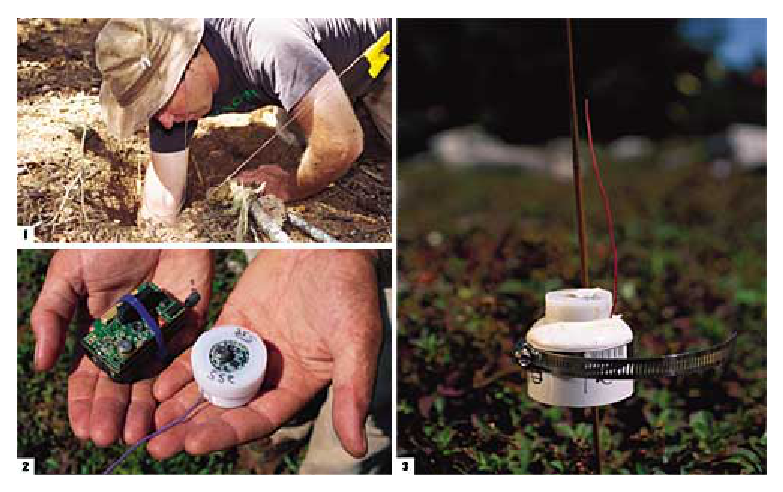
\includegraphics[width=0.4\textwidth]{0404birdf4_123}}
\;
	\subfloat[]{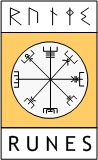
\includegraphics[width=0.1\textwidth]{runes_logo}}
\end{figure}
\end{block}
\end{frame}
%
\begin{frame}{Motivation}
\begin{figure}
  \centering
    \subfloat{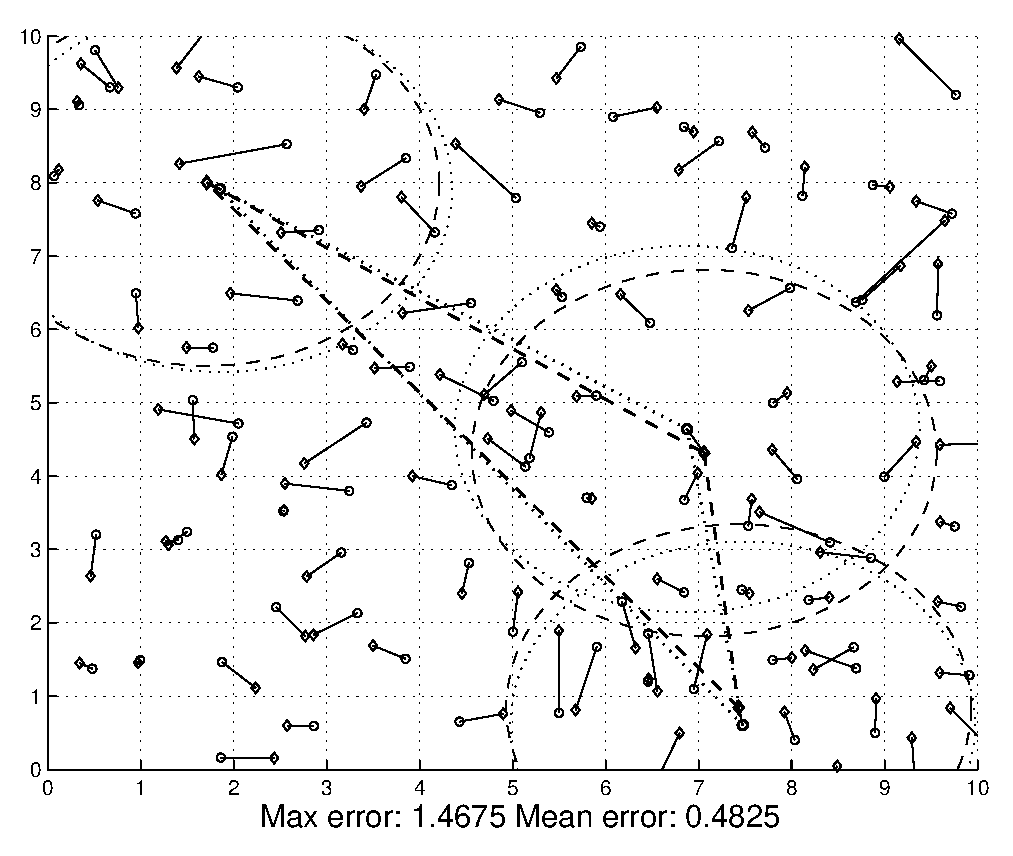
\includegraphics[width=0.32\textwidth]{motivation/plot1}}
    \subfloat{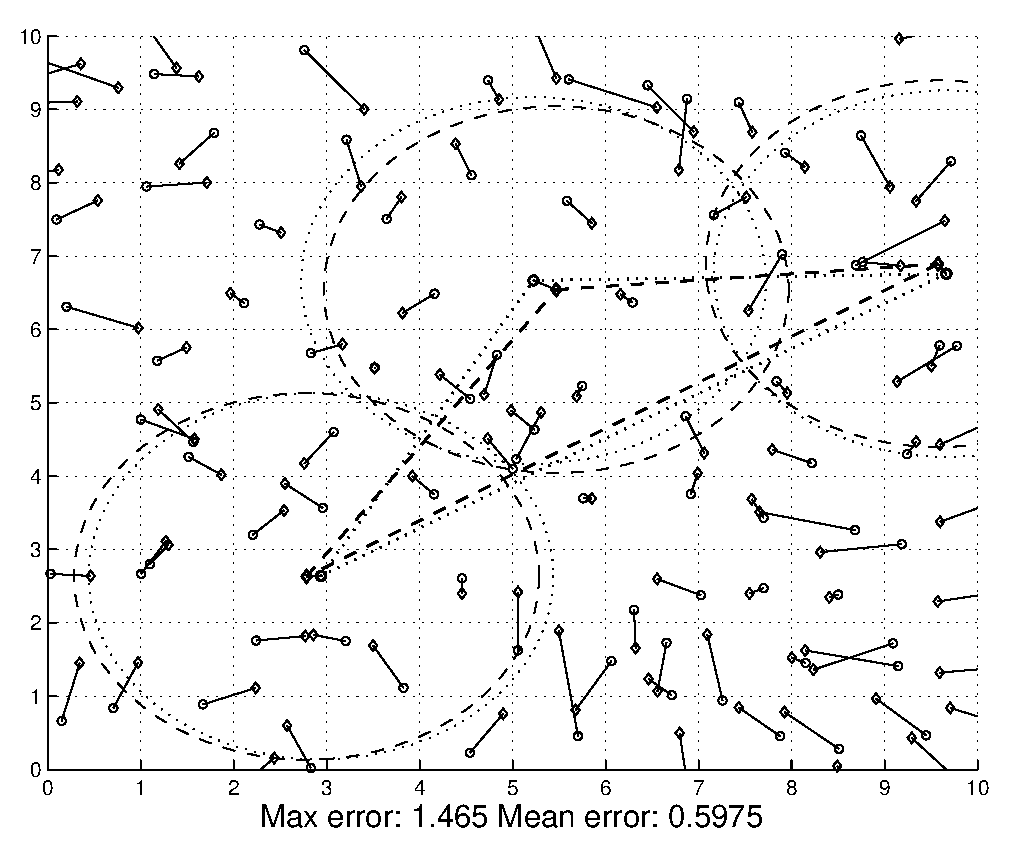
\includegraphics[width=0.32\textwidth]{motivation/plot2}}
	\\
    \subfloat{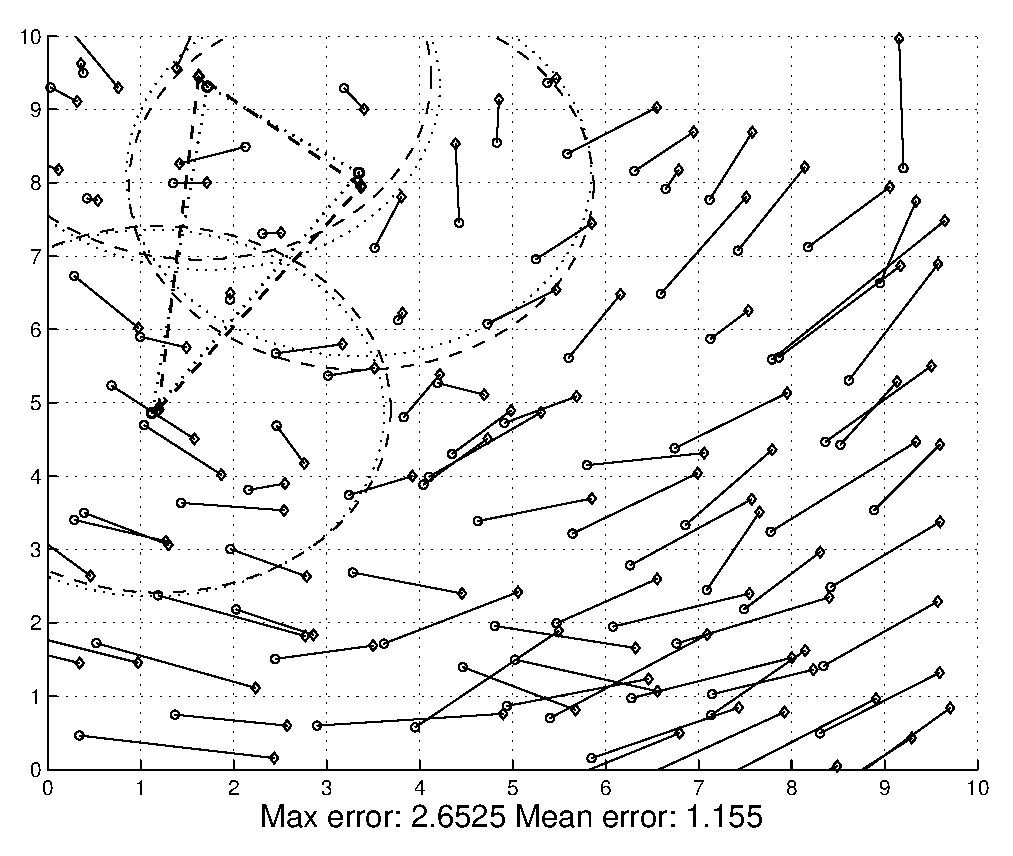
\includegraphics[width=0.32\textwidth]{motivation/plot3}}
    \subfloat{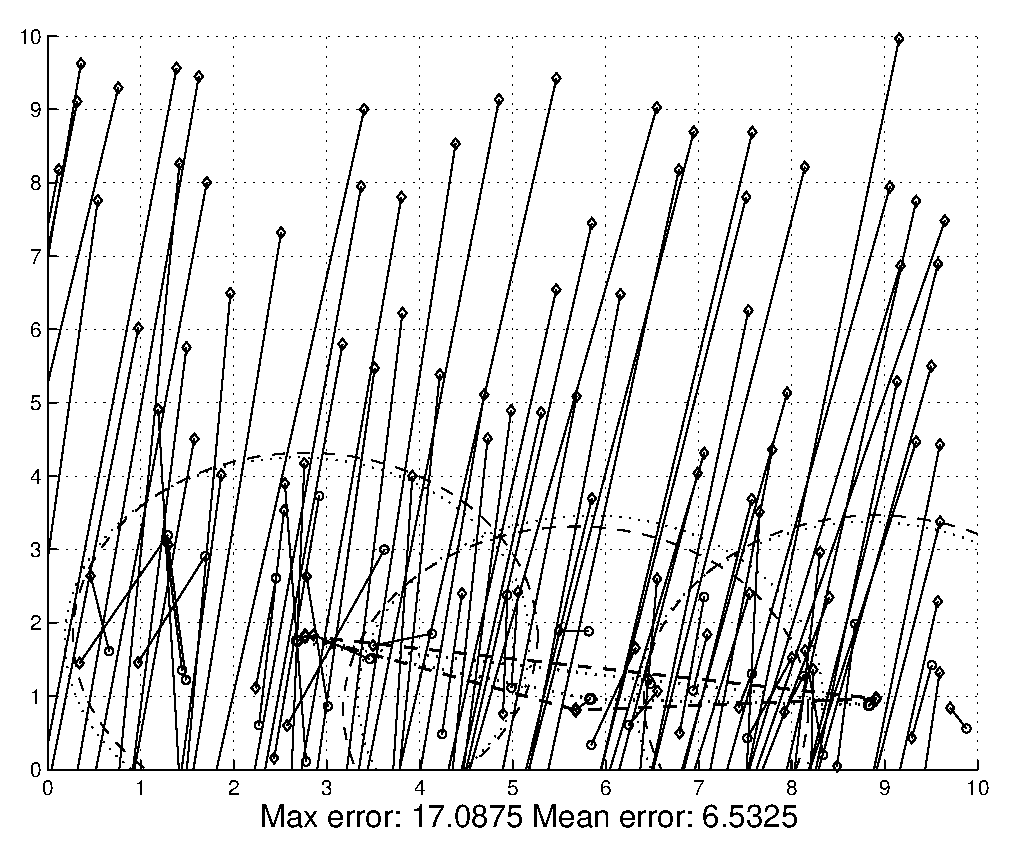
\includegraphics[width=0.32\textwidth]{motivation/plot4}}
\end{figure}
\end{frame}

\begin{frame}{The Basics}
\begin{block}{What are we actually doing?}
\begin{figure}
	\centering	
		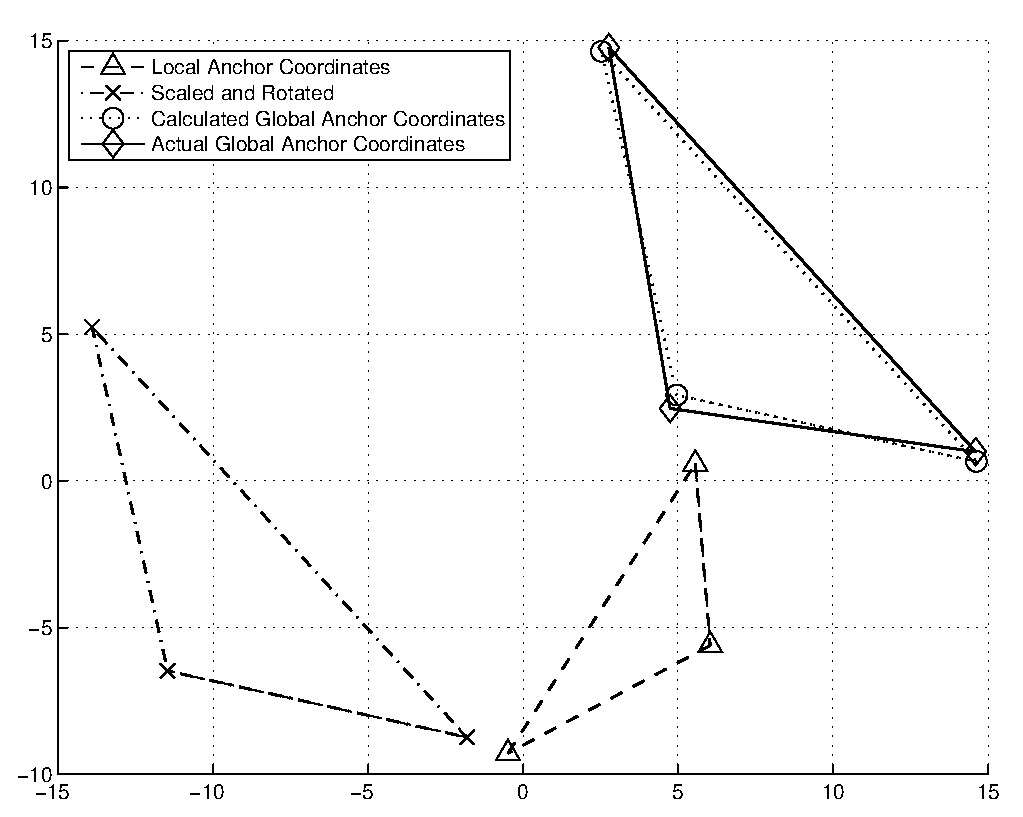
\includegraphics[width=0.7\textwidth]{SampleAnchors}
		\caption{Procrustes Analysis}
\end{figure}
\end{block}
\end{frame}

\begin{frame}{The Worst Case}
\begin{block}{What does it look like}
\begin{figure}
	\centering
		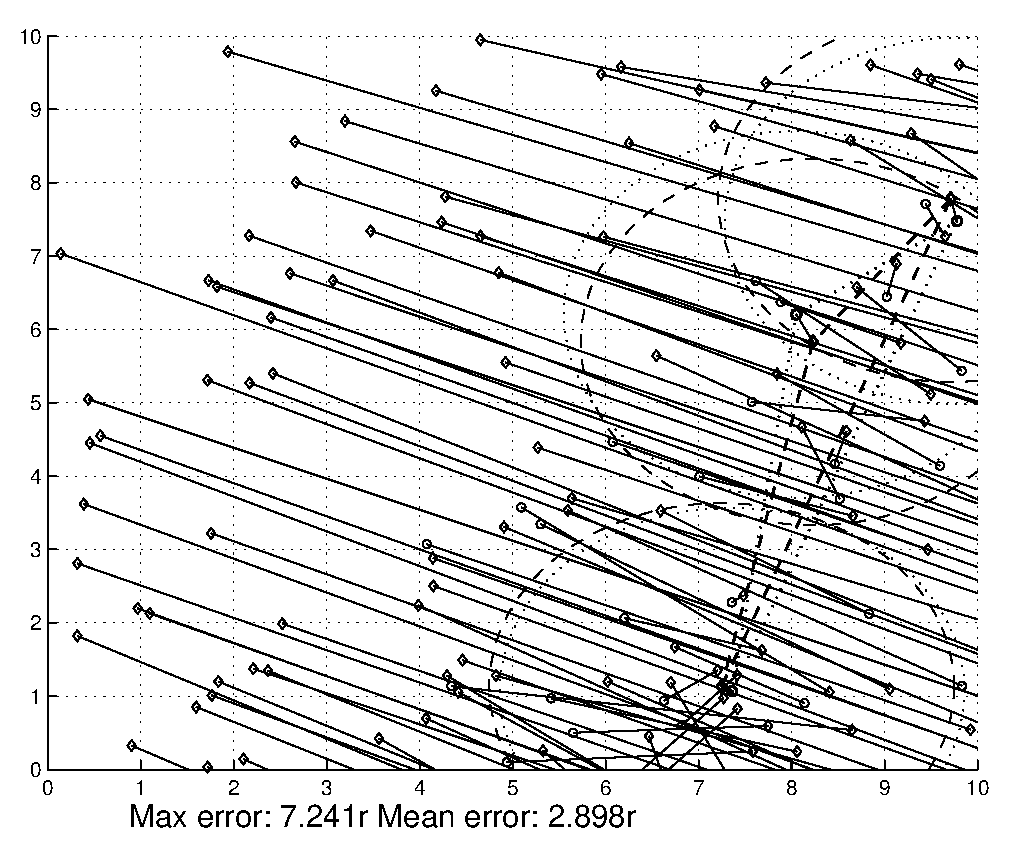
\includegraphics[width=0.7\textwidth]{AS6NetworkDiff9}
		\caption{A really bad result}
\end{figure}
\end{block}
\end{frame}

\begin{frame}{The Worst Case}
\begin{block}{Avoiding it}
\begin{figure}
  \centering
	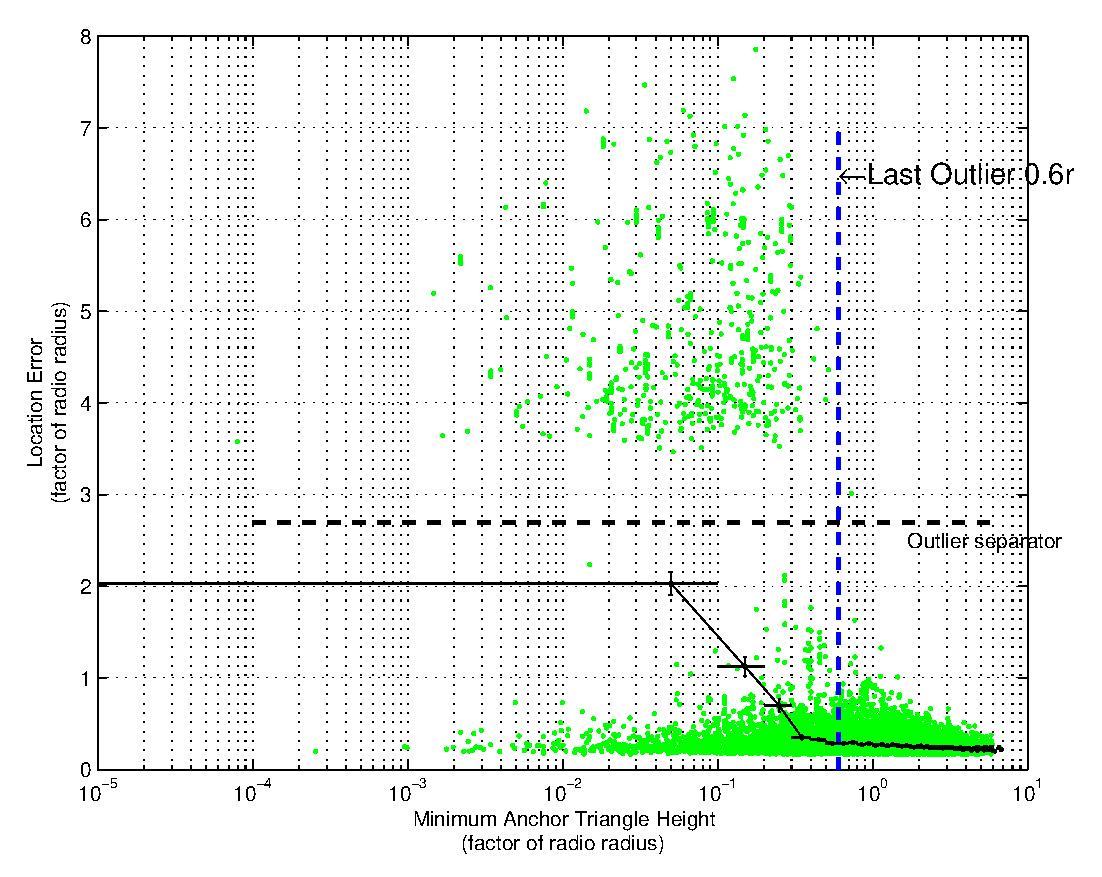
\includegraphics[width=0.6\textwidth]{HeightIndicator_square}
	\caption{Minimum anchor triangle heights, with confidence intervals grouped in intervals of 0.1r}	
\end{figure}
\end{block}
\end{frame}

\begin{frame}{The Normal Case}
\begin{block}{Making the best of it}
\begin{figure}
  \centering
	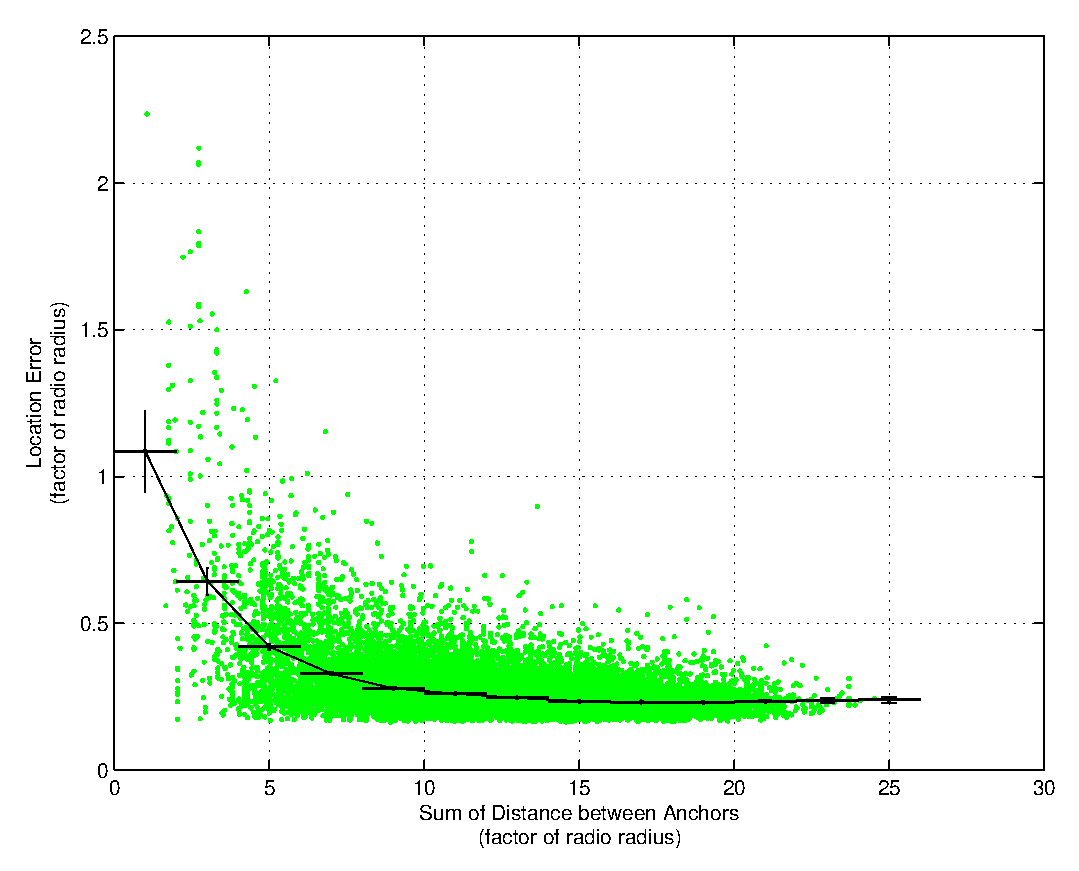
\includegraphics[width=0.6\textwidth]{SumOfDistanceIndicator_square}
	\caption[Sum of distance between anchors vs. location error]{Sum of distance between anchors vs. location error for 20 random square 20-by-20 unit networks with 400 nodes, 5,000 anchor sets each, and a radio range of 2.5 units, excluding outliers}
\end{figure}
\end{block}
\end{frame}

\begin{frame}
\centerline{The End}
\end{frame}
% End of slides
\end{document}